\documentclass[a4paper, 14pt]{extarticle}
\usepackage{float}
% Поля
%--------------------------------------
\usepackage{geometry}
\geometry{a4paper,tmargin=2cm,bmargin=2cm,lmargin=3cm,rmargin=1cm}
%--------------------------------------


%Russian-specific packages
%--------------------------------------
\usepackage[T2A]{fontenc}
\usepackage[utf8]{inputenc}
\usepackage[english, main=russian]{babel}
%--------------------------------------

\usepackage{textcomp}

% Красная строка
%--------------------------------------
\usepackage{indentfirst}
%--------------------------------------


%Graphics
%--------------------------------------
\usepackage{graphicx}
\graphicspath{ {./images/} }
\usepackage{wrapfig}
%--------------------------------------

% Полуторный интервал
%--------------------------------------
\linespread{1.3}
%--------------------------------------

%Выравнивание и переносы
%--------------------------------------
% Избавляемся от переполнений
\sloppy
% Запрещаем разрыв страницы после первой строки абзаца
\clubpenalty=10000
% Запрещаем разрыв страницы после последней строки абзаца
\widowpenalty=10000
%--------------------------------------

%Списки
\usepackage{enumitem}

%Подписи
\usepackage{caption}

%Гиперссылки
\usepackage{hyperref}

\hypersetup {
	unicode=true
}

%Рисунки
%--------------------------------------
\DeclareCaptionLabelSeparator*{emdash}{~--- }
\captionsetup[figure]{labelsep=emdash,font=onehalfspacing,position=bottom}
%--------------------------------------

\usepackage{tempora}

%Листинги
%--------------------------------------
\usepackage{listings}
\lstset{
  basicstyle=\ttfamily\footnotesize,
  %basicstyle=\footnotesize\AnkaCoder,        % the size of the fonts that are used for the code
  breakatwhitespace=false,        % sets if automatic breaks shoulbd only happen at whitespace
  breaklines=true,                 % sets automatic line breaking
  captionpos=t,                    % sets the caption-position to bottom
  inputencoding=utf8,
  frame=single,                    % adds a frame around the code
  keepspaces=true,                 % keeps spaces in text, useful for keeping indentation of code (possibly needs columns=flexible)
  keywordstyle=\bf,       % keyword style
  numbers=left,                    % where to put the line-numbers; possible values are (none, left, right)
  numbersep=5pt,                   % how far the line-numbers are from the code
  xleftmargin=25pt,
  xrightmargin=25pt,
  showspaces=false,                % show spaces everywhere adding particular underscores; it overrides 'showstringspaces'
  showstringspaces=false,          % underline spaces within strings only
  showtabs=false,                  % show tabs within strings adding particular underscores
  stepnumber=1,                    % the step between two line-numbers. If it's 1, each line will be numbered
  tabsize=2,                       % sets default tabsize to 8 spaces
  title=\lstname                   % show the filename of files included with \lstinputlisting; also try caption instead of title
}
%--------------------------------------

%%% Математические пакеты %%%
%--------------------------------------
\usepackage{amsthm,amsfonts,amsmath,amssymb,amscd}  % Математические дополнения от AMS
\usepackage{mathtools}                              % Добавляет окружение multlined
\usepackage[perpage]{footmisc}
%--------------------------------------

%--------------------------------------
%			НАЧАЛО ДОКУМЕНТА
%--------------------------------------

\begin{document}

%--------------------------------------
%			ТИТУЛЬНЫЙ ЛИСТ
%--------------------------------------
\begin{titlepage}
\thispagestyle{empty}
\newpage


%Шапка титульного листа
%--------------------------------------
\vspace*{-60pt}
\hspace{-65pt}
\begin{minipage}{0.3\textwidth}
\hspace*{-20pt}\centering

\includegraphics[width=\textwidth]{emblem}
\end{minipage}
\begin{minipage}{0.67\textwidth}\small \textbf{
\vspace*{-0.7ex}
\hspace*{-6pt}\centerline{Министерство науки и высшего образования Российской Федерации}
\vspace*{-0.7ex}
\centerline{Федеральное государственное бюджетное образовательное учреждение }
\vspace*{-0.7ex}
\centerline{высшего образования}
\vspace*{-0.7ex}
\centerline{<<Московский государственный технический университет}
\vspace*{-0.7ex}
\centerline{имени Н.Э. Баумана}
\vspace*{-0.7ex}
\centerline{(национальный исследовательский университет)>>}
\vspace*{-0.7ex}
\centerline{(МГТУ им. Н.Э. Баумана)}}
\end{minipage}
%--------------------------------------

%Полосы
%--------------------------------------
\vspace{-25pt}
\hspace{-35pt}\rule{\textwidth}{2.3pt}

\vspace*{-20.3pt}
\hspace{-35pt}\rule{\textwidth}{0.4pt}
%--------------------------------------

\vspace{1.5ex}
\hspace{-35pt} \noindent \small ФАКУЛЬТЕТ\hspace{80pt} <<Информатика и системы управления>>

\vspace*{-16pt}
\hspace{47pt}\rule{0.83\textwidth}{0.4pt}

\vspace{0.5ex}
\hspace{-35pt} \noindent \small КАФЕДРА\hspace{50pt} <<Теоретическая информатика и компьютерные технологии>>

\vspace*{-16pt}
\hspace{30pt}\rule{0.866\textwidth}{0.4pt}

\vspace{11em}

\begin{center}
\Large {\bf Летучка № 1 } \\
\large {\bf по курсу <<Численные методы линейной алгебры>>} \\
\large <<Реализация метода прогонки и оценка погрешностей
вычислений>>
\end{center}\normalsize

\vspace{8em}


\begin{flushright}
  {Студент группы ИУ9-71Б Баев Д.А \hspace*{15pt}\\
  \vspace{2ex}
  Преподаватель Посевин Д. П.\hspace*{15pt}}
\end{flushright}

\bigskip

\vfill


\begin{center}
\textsl{Москва 2023}
\end{center}
\end{titlepage}
%--------------------------------------
%		КОНЕЦ ТИТУЛЬНОГО ЛИСТА
%--------------------------------------

\renewcommand{\ttdefault}{pcr}

\setlength{\tabcolsep}{3pt}
\newpage
\setcounter{page}{2}

\section{Задание}\label{Sect::task}
1. Реализовать метод прогонки для A · x = f; A принадлежит R100×100; f, x принадлежит R100; A -
трехдиагональная матрица.

2. Найти относительные погрешности метода прогонки в сравнении с идеальным решением, простейшего метода Гаусса в сравнении с идеальным
решением и библиотечного метода в сравнении с идеальыом решением.
Идеальное решение брать как в лабораторной №2.
\newpage
\section{Исходный код}

Исходный код программы представлен в листингах~\ref{lst:code1}--~\ref{lst:code4}.

\begin{figure}[H]
\begin{lstlisting}[language={},caption={Реализация метода прогонки},label={lst:code1}]
def thomas(A, b):
    n = len(b)

    alpha = np.zeros(shape=(n, ))
    beta = np.zeros(shape=(n, ))

    alpha[0] = -A[0][1] / A[0][0]
    beta[0] = b[0] / A[0][0]

    for i in range(1, n):
        if i == n - 1:
            alpha[i] = 0
            denominator = A[i][i] + A[i][i - 1] * alpha[i - 1]
        else:
            denominator = A[i][i] + A[i][i - 1] * alpha[i - 1]
            alpha[i] = -A[i][i + 1] / denominator
        beta[i] = (b[i] - A[i][i - 1] * beta[i - 1]) / denominator
    x = np.zeros(shape=(n, ))
    x[n - 1] = beta[n - 1]
    for i in range(n - 2, -1, -1):
        x[i] = alpha[i] * x[i + 1] + beta[i]
    return x
\end{lstlisting}
\end{figure}

\begin{figure}[H]
\begin{lstlisting}[language={},caption={Реализация вспомогательных функций},label={lst:code2}]
def norm(vector):
    return np.sqrt(sum(x**2 for x in vector))

def mul_matrix_by_vector(matrix, vector):
    assert len(matrix[0]) == len(vector)
    return np.array([sum(matrix[i][j] * vector[j] for j in range(len(vector))) for i in range(len(matrix))])


def gauss(A, b):
    n = len(A)
    A = deepcopy(A)
    b = deepcopy(b)

    for i in range(n):
        if A[i][i] == 0:
            for j in range(i + 1, n):
                if A[j][i] != 0:
                    A[i], A[j] = A[j], A[i]
                    break

        for j in range(i + 1, n):
            f = A[j][i] / A[i][i]
            A[j] -= f * A[i]
            b[j] -= f * b[i]

    x = np.zeros(shape=(n, ))

    for i in range(n - 1, -1, -1):
        x[i] = b[i] / A[i][i]
        for j in range(i - 1, -1, -1):
            b[j] -= A[j][i] * x[i]

    return np.array(x)

def random_tridiagonal_matrix(a, b, n):
    matrix = np.zeros((n, n))
    for i in range(n):
        matrix[i][i] = random.uniform(a, b)
        if i > 0:
            matrix[i][i-1] = random.uniform(a, b)
        if i < n - 1:
            matrix[i][i+1] = random.uniform(a, b)

    return matrix
\end{lstlisting}
\end{figure}

\begin{figure}[H]
\begin{lstlisting}[language={},caption={Оценка погрешностей},label={lst:code3}]
A = random_tridiagonal_matrix(0, 10, 100)
x = np.random.uniform(low=0, high=10, size=100)
b = mul_matrix_by_vector(A, x)

x_gauss = gauss(A, b)
x_thomas = thomas(A, b)
x_np = np.linalg.solve(A, b)

relative_gauss = norm(x - x_gauss) / norm(x) * 100
relative_thomas = norm(x - x_thomas) / norm(x) * 100
relative_np = norm(x - x_np) / norm(x) * 100

print(norm(x - x_gauss), relative_gauss)
print(norm(x - x_thomas), relative_thomas)
print(norm(x - x_np), relative_np)
\end{lstlisting}
\end{figure}

\section{Результаты}

Результаты оценки погрешностей приведены на рисунках~\ref{fig:img1}-~\ref{fig:img3}.

\begin{figure}[H]
\centering
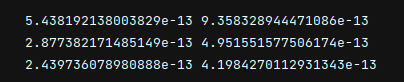
\includegraphics[width=0.8\textwidth]{images/res1.png}
\caption{Результат оценки погрешностей}
\label{fig:img1}
\end{figure}


\begin{figure}[H]
\centering
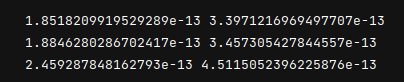
\includegraphics[width=0.8\textwidth]{images/res2.png}
\caption{Результат оценки погрешностей}
\label{fig:img2}
\end{figure}


\begin{figure}[H]
\centering
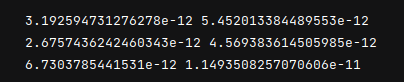
\includegraphics[width=0.8\textwidth]{images/res3.png}
\caption{Результат оценки погрешностей}
\label{fig:img3}
\end{figure}


\section{Выводы}
В рамках данной лабораторной работы был использован метод прогонки для решения системы линейных уравнений, где матрица была трехдиагональной. Было проведено сравнение относительной погрешности этого метода с аналогичными результатами, полученными при использовании метода Гаусса и функции из библиотеки Numpy. Поскольку метод прогонки специализирован именно для трехдиагональных матриц, его результаты оказались более точными и эффективными по сравнению с методом Гаусса.
\end{document}